\begin{frame}{Getting Things Done}
  \begin{center}
    
\includegraphics[height=6cm]{img/gtd.png}
  \end{center}
\end{frame}

\begin{frame}{Getting Things Done}
  \begin{block}{Characteristics}
    \begin{itemize}
      \item Task management system.
      \item More stuff in head, harder to decide what needs attention.
      \item Dump your mental clutter into an external system.
      \item Focus on right things at right times.
    \end{itemize}
  \end{block}
\end{frame}

\begin{frame}{Getting Things Done}
  \begin{block}{5 steps}
    \begin{itemize}
      \item Capture: mind $\rightarrow$ inbox.
      \item Clarify: inbox $\rightarrow$ action steps.
      \item Organize: action steps $\rightarrow$ calendar, delegate, refernece, my-tasks.
      \item Review: daily (small) and weekly (large) lists update.
      \item Engage: you know what and when.
    \end{itemize}
  \end{block}
\end{frame}

\begin{frame}{Getting Things Done}
  \begin{block}{GTD diagram}
    \begin{center}
      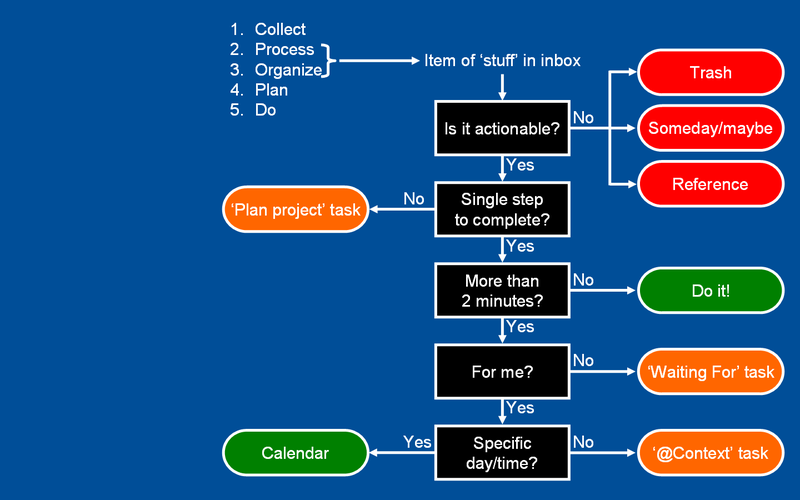
\includegraphics[height=6cm]{img/gtd-diagram.png}
    \end{center}
  \end{block}
\end{frame}

\begin{frame}{Getting Things Done}
  \begin{block}{1. Capture}
    \begin{itemize}
      \item Collect ideas.
      \item An inbox. % dynamic list, easy to access, always available
      \item Several lists. % life goals, medium long, 1-2 years, current projects
      \item Reference.
      \item Maybe.
      \item Delegated.
      \item Agendas.
      \item Calendar.
    \end{itemize}
  \end{block}
\end{frame}

\begin{frame}{Getting Things Done}
  \begin{block}{2. Clarify}
    \begin{itemize}
      \item Less than 2 mintues $\rightarrow$ do it right away.
      \item Can it be delegated $\rightarrow$ assign it to someone else.
      \item Non-actionable item $\rightarrow$ reference. % files, documents, contact info
      \item Specific date and time $\rightarrow$ calendar.
      \item No longer needed/actionable $\rightarrow$ delete it.
      \item More than 1 step $\rightarrow$ create a project and identify the first "next action". % get a hair cut => find a barber shop in my area which is open at 18:00
      \item Actionable items should contain all necessary info. % "hair" vs "call ABC on +31677711122, ask for ..."
    \end{itemize}
  \end{block}
\end{frame}

\begin{frame}{Getting Things Done}
  \begin{block}{3. Organize}
    \begin{itemize}
      \item One-off tasks (special project): take longer than 2min, but require just one step.
      \item Projects: all items that require 2+ steps.
      \item Areas of focus (categories of projects).
      \item Next actions: first items of all projects.
      \item Tasks with due date: schedule them.
      \item Agendas (special project): create a sub-project for each person.
      \item Reference materials: e. g. documents, attach them to tasks.
      \item Waiting for: delegated items.
      \item Some day / maybe: ideas for future
      \item Tasks that can be delegated: delegate.
      \item Contexts: tools, places or people you need. % offline, 15m-or-less
    \end{itemize}
  \end{block}
\end{frame}

\begin{frame}{Getting Things Done}
  \begin{block}{My door}
    \begin{center}
      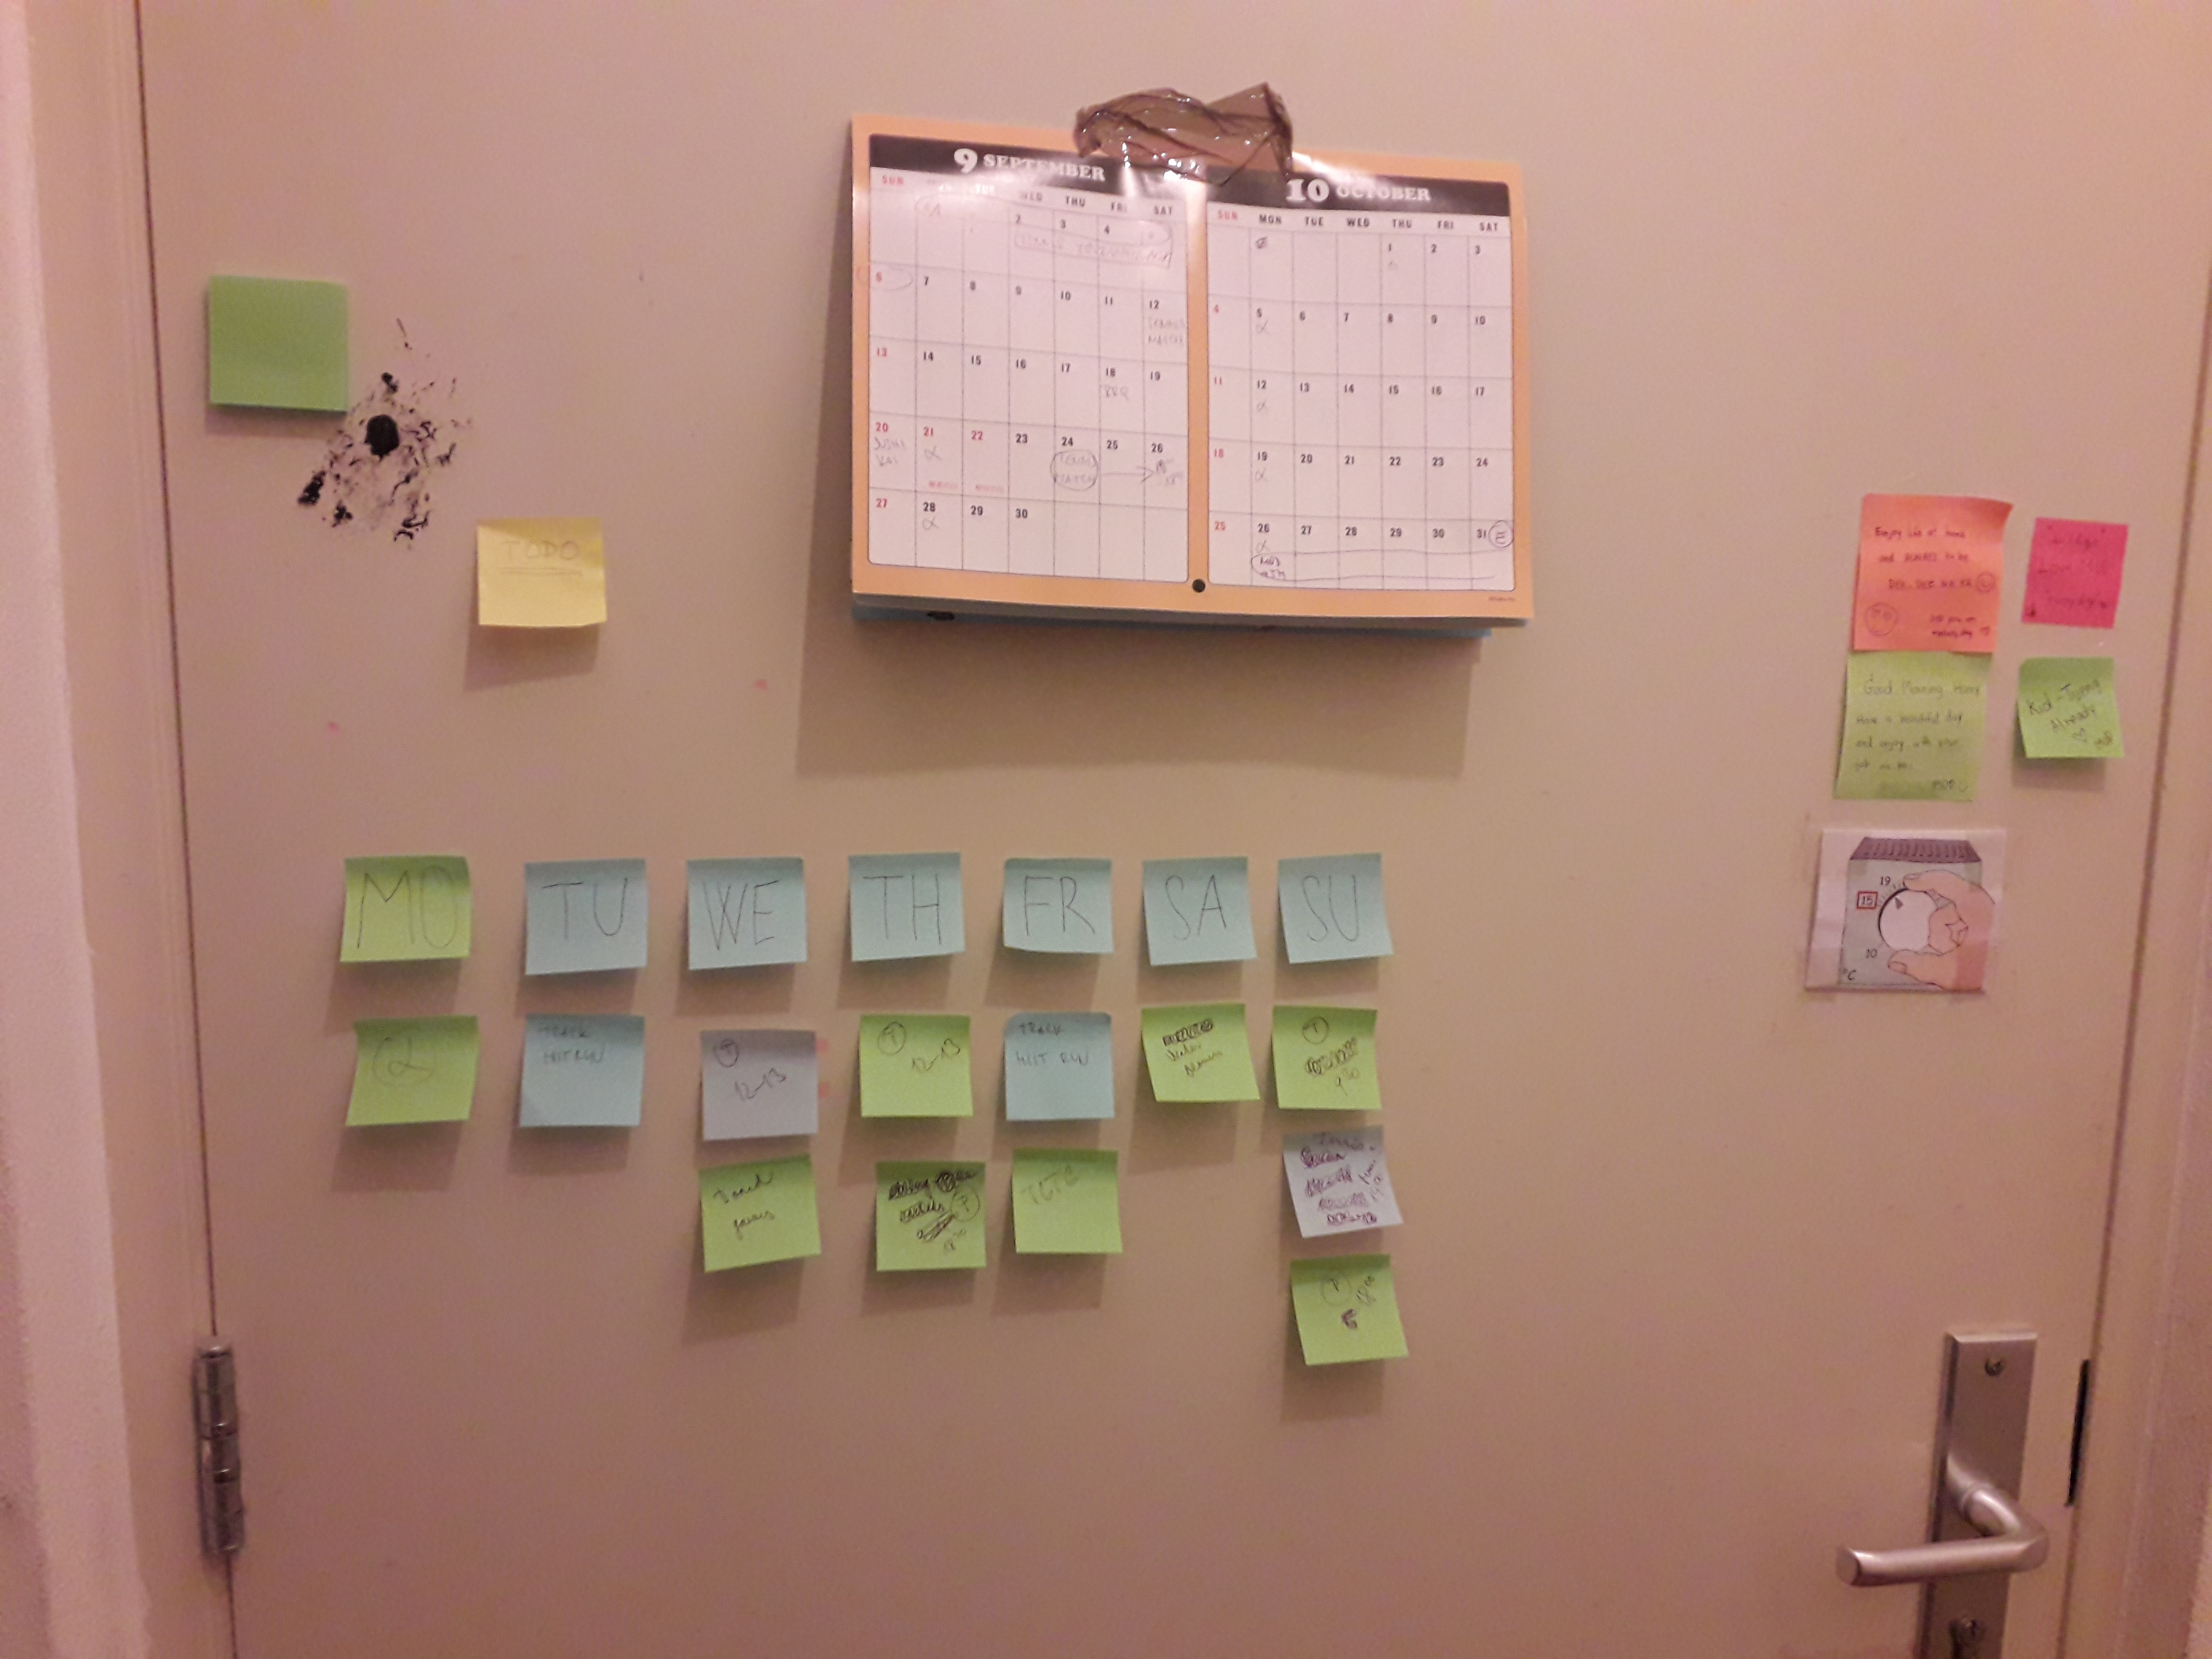
\includegraphics[height=6cm]{img/week-agenda-01.jpg}
    \end{center}
  \end{block}
\end{frame}

\begin{frame}{Getting Things Done}
  \begin{block}{My door}
    \begin{center}
      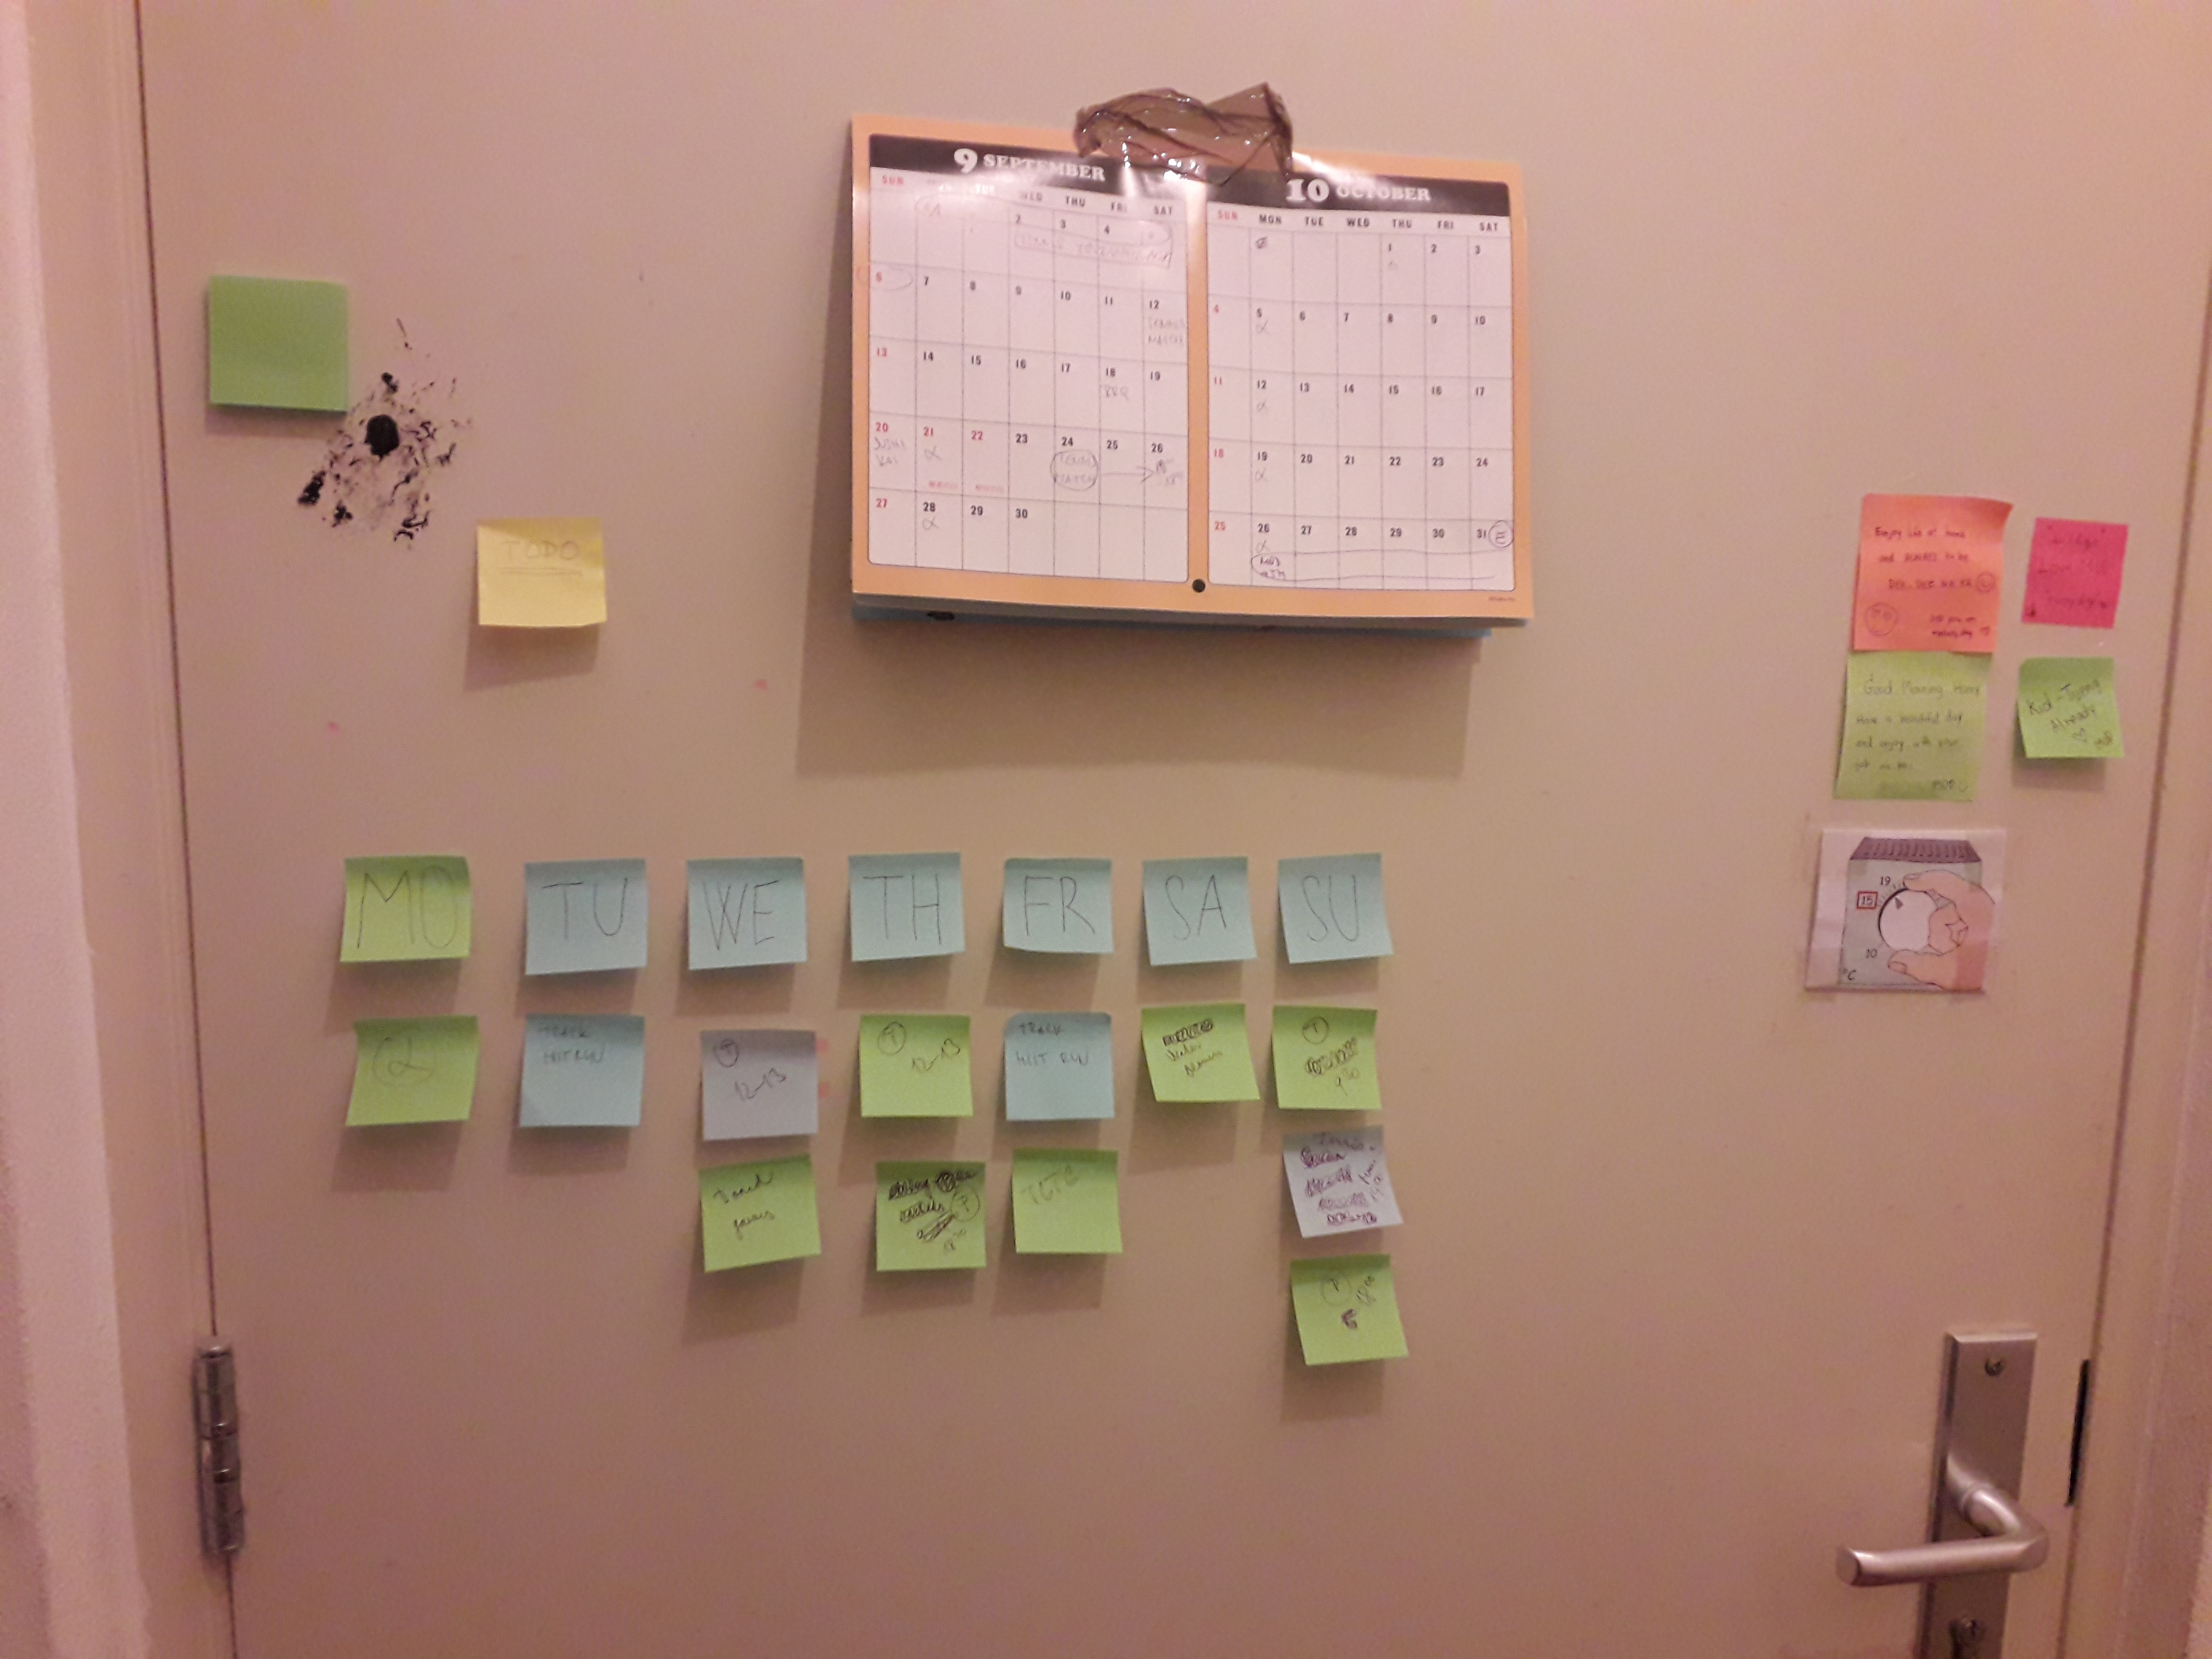
\includegraphics[height=6cm]{img/week-agenda-02.jpg}
    \end{center}
  \end{block}
\end{frame}

\begin{frame}{Getting Things Done}
  \begin{block}{Our board}
    \begin{center}
      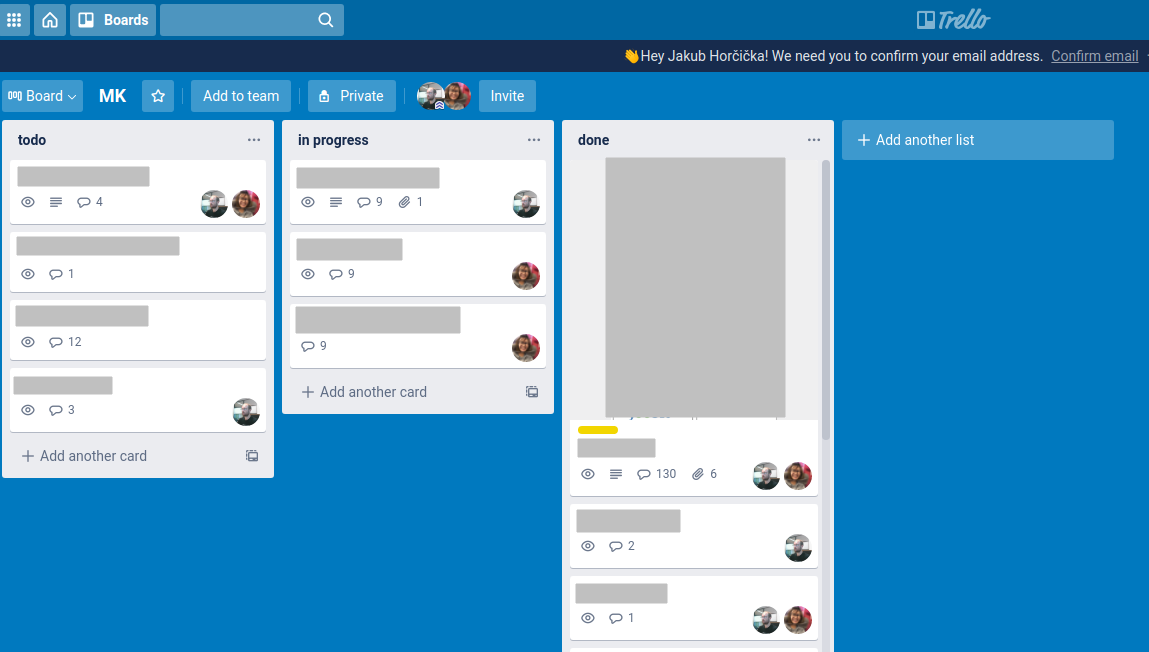
\includegraphics[height=6cm]{img/trello.png}
    \end{center}
  \end{block}
\end{frame}

\begin{frame}{Getting Things Done}
  \begin{block}{My phone}
    \begin{center}
      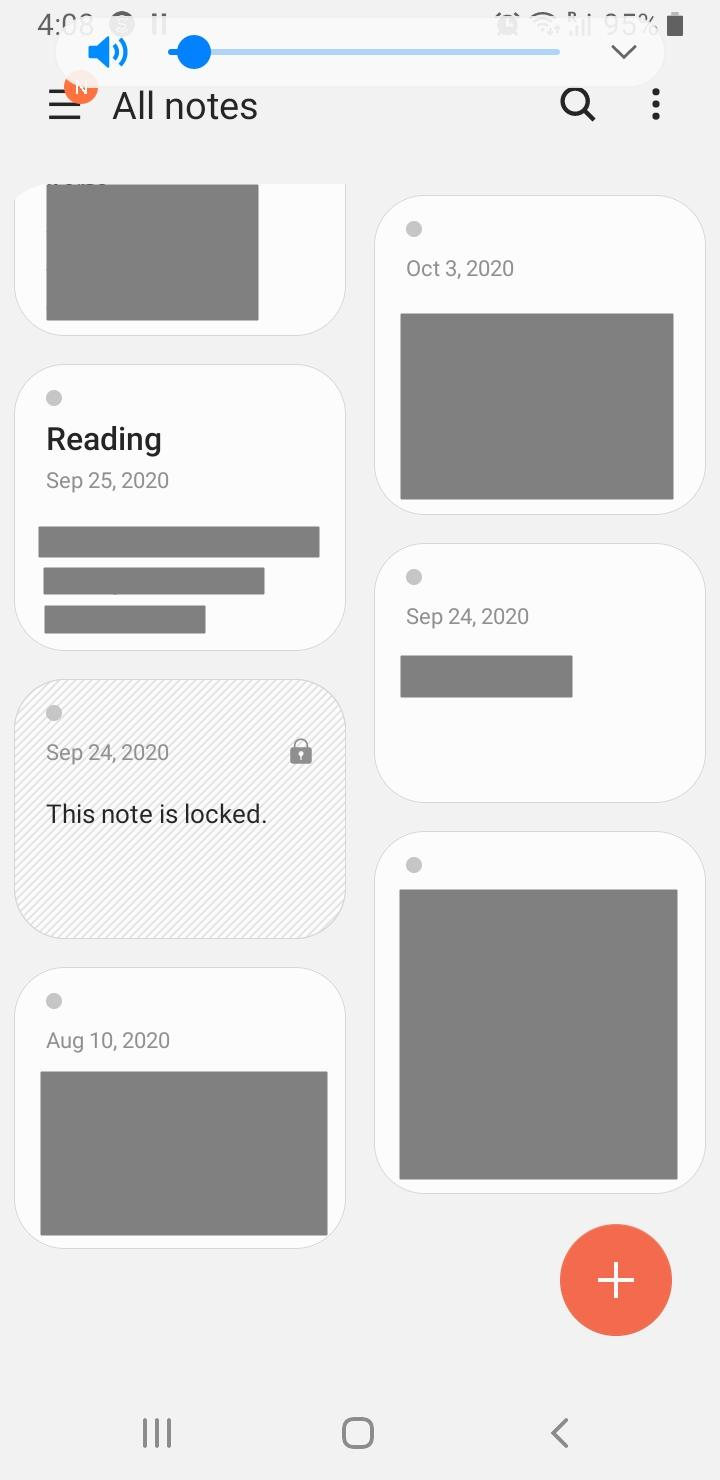
\includegraphics[height=6cm]{img/phone-notes.jpg}
    \end{center}
  \end{block}
\end{frame}

\begin{frame}{Getting Things Done}
  \begin{block}{4. Review}
    \begin{itemize}
      \item Clean your inbox every day (or week). 
      \item Once a week schedule time to organize tasks.
    \end{itemize}
  \end{block}
\end{frame}

\begin{frame}{Getting Things Done}
  \begin{block}{5. Engage}
    \begin{itemize}
      \item We have concrete, actionable items.
      \item We can answer: "what should I be doing right now?".
    \end{itemize}
  \end{block}
\end{frame}

